\documentclass[9pt,twocolumn,letterpaper]{extarticle}
\usepackage[margin=0.5in,columnsep=0.22in]{geometry}
\usepackage{times}
\usepackage{amsmath,amssymb}
\usepackage{booktabs}
\usepackage{xcolor}
\usepackage{graphicx}
\usepackage[ruled,noline,linesnumbered]{algorithm2e}
\usepackage{titlesec}
\usepackage[hidelinks]{hyperref}
\usepackage{caption}
\usepackage{float}
\captionsetup{font=footnotesize,skip=3pt}
\titlespacing*{\section}{0pt}{4pt}{2pt}
\titleformat{\section}{\normalsize\bfseries}{\thesection}{0.5em}{}
\setlength{\parskip}{1pt}
\setlength{\abovedisplayskip}{3pt}\setlength{\belowdisplayskip}{3pt}
\setlength{\abovedisplayshortskip}{2pt}\setlength{\belowdisplayshortskip}{2pt}
\SetAlFnt{\footnotesize}
\newcommand{\tbd}[1]{\textcolor{red}{#1}}
\pagestyle{empty}
\raggedbottom

\begin{document}

\twocolumn[{%
\centering
{\large\bfseries Checkpoint 3: An Order-Controlled Search Agent for Misstatement-Risk Screening}\\[2pt]
{\small Ryan Khan \quad IDAI-780, Fall 2026 \quad Instructor: Zhiqiang Tao \quad Code: \tbd{github.com/\textless user\textgreater/fraud-cot-search-agent}}\\[3pt]
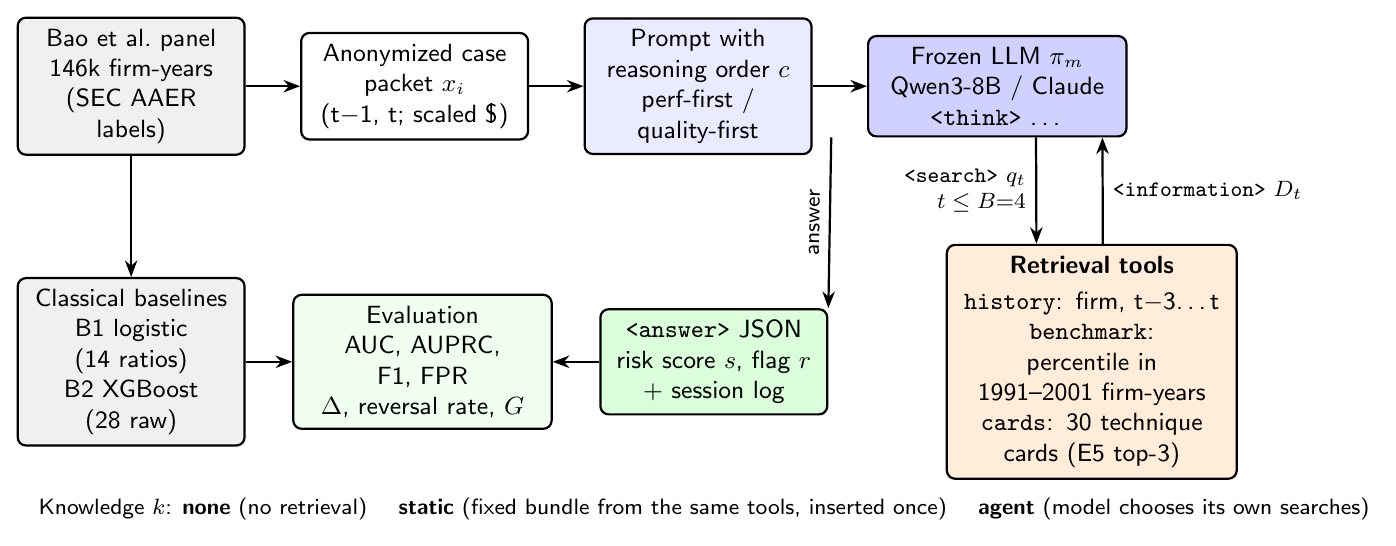
\includegraphics[width=0.66\textwidth]{../assets/framework.png}\\[-2pt]
{\footnotesize Figure 1: Framework. A frozen LLM reasons in order $c$ and, in the agent setting, issues up to $B{=}4$ searches to three leakage-safe tools before answering; outputs are scored with the same metrics as the classical baselines.}\\[4pt]
}]

\section{Formulation}
\textbf{Data and task.} We use the Bao et al.\ \cite{bao2020} panel of U.S.\ firm-years with SEC AAER labels $y_i\in\{0,1\}$. Splits are temporal: train 1991--2001, test 2003--2008, with a two-year gap and serial-fraud relabelling. Case $i$ is an anonymized packet $x_i$ with 28 items for years $t{-}1,t$ and 14 ratios. Firm ID and calendar years are removed, and dollar amounts are multiplied by a random constant $\lambda_i\in[0.5,2]$.

\textbf{Inference model.} A frozen LLM $\pi_m$ ($m\in\{$Qwen3-8B, Claude Sonnet 5.5$\}$) runs under reasoning order $c\in\{\mathrm{D},\mathrm{P},\mathrm{Q}\}$: direct; \emph{performance-first} (growth, margins, ROA, the headline story); and \emph{quality-first} (accruals, cash, receivables, inventory, soft assets). The two CoT prompts contain the same words in a different order. Knowledge is $k\in\{\varnothing,\mathrm{S},\mathrm{A}\}$: none, static bundle, or search agent. Following Search-R1 \cite{searchr1}, without RL, the agent produces
\begin{equation}
\pi_m(\tau\mid x_i;c)=\prod_{t=1}^{T}\pi_m\!\left(t_t,q_t\mid x_i,c,\tau_{<t}\right),\quad T\le B,
\end{equation}
where $t_t$ is a \texttt{<think>} step and $q_t$ a \texttt{<search>} call to one of three tools. \texttt{history} returns the firm's own $t{-}3..t$ values scaled by $\lambda_i$. \texttt{benchmark} returns the percentile of a ratio among 1991--2001 firm-years. \texttt{cards} returns the top-3 of 30 technique cards,
\begin{equation}
D_t=\operatorname{TopK}_{d\in\mathcal{T}}\cos\big(\phi(q_t),\phi(d)\big),
\end{equation}
where $\phi$ is the E5 encoder. Each $D_t$ is inserted inside \texttt{<information>}; the model conditions on it but does not generate it. The answer gives a risk score $s_i^{m,c,k}\in[0,100]$ and a red flag $r_i=\mathbb{1}[s_i\ge\theta_{m,c,k}]$, with $\theta$ chosen to maximize F1 on a disjoint dev split (2000--01 cases).

\textbf{Hypotheses.} \emph{H1 (order bias):} $\Delta_i^{m,k}=s_i^{m,\mathrm{P},k}-s_i^{m,\mathrm{Q},k}$ is negative, i.e.\ reasoning that starts from performance anchors on the headline numbers. We report mean $\Delta$, $|\Delta|$, the red-flag reversal rate $\rho$, and a Wilcoxon signed-rank test. \emph{H3 (knowledge):} $G^{m,c}=\mathrm{AUPRC}(\mathrm{A})-\mathrm{AUPRC}(\mathrm{S})>0$, and $|\Delta^{\mathrm{A}}|<|\Delta^{\varnothing}|$. The agent's own queries can show the mechanism: we measure the share of lookups aimed at quality items under each order.

\begin{algorithm}[h]
\caption{Order-controlled search agent (batched)}
\KwIn{cases $\{x_i\}$, model $\pi_m$, order $c$, budget $B{=}4$}
$h_i\leftarrow\textsc{Prompt}(x_i,c)$ for all $i$; active $\leftarrow$ all\;
\While{active $\neq\varnothing$ and step $< B{+}4$}{
 $y_i\leftarrow\pi_m(h_i)$ until \texttt{</search>}$\,|\,$\texttt{</answer>} \tcp*{batched}
 \ForEach{active $i$}{
 \uIf{\texttt{<answer>} in $y_i$}{close $i$}
 \uElseIf{$(tool,q)\leftarrow\textsc{Parse}(y_i)$, $n_i<B$}{$D\leftarrow\textsc{Tool}(tool,q)$; $h_i\mathrel{+}=y_i\|\texttt{<information>}D\texttt{</information>}$; log $(q,\mathrm{IDs}(D))$; $n_i{+}{+}$}
 \lElse{``rethink'' once (or budget used): force \texttt{<answer>}}
}}
\Return $\textsc{ParseJSON}(h_i)$ for all $i$\;
\end{algorithm}

\section{Comparison to Baselines}
\begin{table}[H]
\centering\footnotesize\setlength{\tabcolsep}{3.5pt}
\begin{tabular}{llccc}
\toprule
Model & Condition $(c,k)$ & AUC & AUPRC & $|\Delta|$ \\
\midrule
B0 & random & 0.58 & 0.57 & -- \\
B1 & logistic, 14 ratios & 0.62 & 0.59 & -- \\
B2 & XGBoost, 28 items & \textbf{0.76} & \textbf{0.76} & -- \\
\midrule
Qwen3-8B & D, $\varnothing$ (CP2 Direct) & \tbd{--} & \tbd{--} & -- \\
 & P\,/\,Q, $\varnothing$ (CoT) & \tbd{--} & \tbd{--} & \tbd{--} \\
 & P\,/\,Q, S (static RAG) & \tbd{--} & \tbd{--} & \tbd{--} \\
 & \textbf{P\,/\,Q, A (agent)} & \tbd{--} & \tbd{--} & \tbd{--} \\
Claude & same grid & \tbd{--} & \tbd{--} & \tbd{--} \\
\bottomrule
\end{tabular}
\caption{The same 60 balanced out-of-sample test cases (30 later-AAER). Values have 95\% case-bootstrap CIs (in repo). On the full test set (35,166 firm-years) B2 reaches AUC 0.725 and AUPRC 0.015 against a prevalence of 0.0074, in line with Bao et al.'s RUSBoost ($\approx$0.71).}
\end{table}
\vspace{-6pt}
\noindent\textbf{Qualitative.} Classical models see only numbers, so order cannot affect them. Static RAG gives every case the same bundle. The agent chooses what to check and every check is logged, so we can ask \emph{why} order matters: does performance-first reasoning lead to fewer quality checks?

\section{Implementation Details}
\textbf{Training (B2).} XGBoost minimizes $\sum_i w_{y_i}\ell(y_i,f(z_i))+\Omega(f)$ with $w_1=n_0/n_1$. Hyperparameters are chosen on fit 1991--97 $\to$ validation 2000--01 over depth $\{3,4,6\}\times$ trees $\{200,400\}$ (learning rate 0.05, row and column subsample 0.8). The selected setting (depth 3, 200 trees) is refit on 1991--2001 with median imputation and 1/99\% winsorizing fit on training rows only. We log per-round log loss, AUC and AUPRC, save checkpoints every 50 rounds, and score the test years once.
\textbf{LLM testing.} Qwen3-8B runs in bf16 with Transformers on one \tbd{A100}, with greedy decoding, built-in thinking off, at most 1{,}024 new tokens per step, and batched lock-step rollouts (16 sessions per batch). Claude runs the same tools through native API tool use at effort low (D) or high (CoT), since it does not write out its reasoning. Static RAG covers 4 history items, 13 ratio benchmarks and the top-6 cards. Every session logs the case, condition, prompt hash, queries, retrieved IDs, malformed or forced flags and raw output. There are 13 unit tests covering the parser, budget cutoff, rethink path, leakage guards, retrieval determinism, prompt symmetry and schema. Uncertainty comes from 1{,}000 case-bootstrap resamples, paired across conditions.

\vspace{-4pt}
{\footnotesize
\begin{thebibliography}{9}\setlength{\itemsep}{0pt}
\bibitem{bao2020} Y.~Bao et al. Detecting accounting fraud in publicly traded U.S.\ firms using a machine learning approach. \emph{J.\ Accounting Research}, 58(1), 2020.
\bibitem{searchr1} B.~Jin et al. Search-R1: Training LLMs to reason and leverage search engines with reinforcement learning. \emph{COLM}, 2025.
\end{thebibliography}}
\end{document}
